\newpage
\section{Morfeas System configuration} \label{sys_conf}
The ``Morfeas System configuration" utility can be accessed from the Morfeas WEB front page from the button with the Morfeas core configuration logo
(
\includegraphics[height=.150in]{../art/morfeas_gear.png}).\\

The ``Morfeas System configuration" utility have three tabs, that are: ``Morfeas System", ``ISOStandards", ``Up/Down Load".
With the ``Morfeas System" tab the user can manipulate the components of the Morfeas system.
The ``ISOStandards" tab, print in a table the current ISOStandards file that is loaded in the server.
The ``Up/Down Load" tab have the necessary utilities for download the current ISOStandard and upload a new one.
Also to get/set the Morfeas configuration and ISOChannels using the Morfeas bundle files (mbl).\\

\noindent At the following subsections will be introduced the operation for each tab of the utility.

\subsection{``Morfeas System"}
At the figure \ref{fig:Morfeas_sys_conf} shown an example of the ``Morfeas System" tab.
The left side have a tree with the currently configured components of the Morfeas system.
The Morfeas System can have up to 16 components, from them one is always occupied by the Morfeas OPC-UA component,
so 15 of them are used configurable.

\begin{figure}[h]
\centering
	\fbox{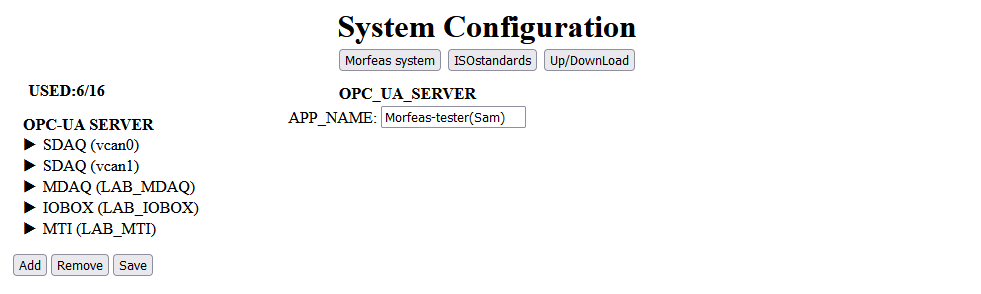
\includegraphics[width=4in,angle=0]{../art/Morfeas_web_if/Morfeas_sys_conf.png}}
	\caption{Morfeas System configuration}
	\label{fig:Morfeas_sys_conf}
\end{figure}

Bellow the components tree are three buttons with command that are for manipulation of the components.
That are: ``Add", ``Remove", ``Save".\\

\noindent The ``Add" button can add a new components, when it is press will show a new window with the ``Add Component" utility
(figure \ref{fig:Morfeas_sys_conf_add_comp}).
The ``Add Component" utility required from the user to choose what type of component will be added, together with the necessary options.\\

\noindent The ``Remove" button will remove from the tree the component which is selected (except from the Morfeas OPC-UA. Which can not be removed).\\

\noindent The ``Save" button will send and apply the modification to the server.\\

The right section of the ``Morfeas System" tab, contains the configuration options of the selected component.
For any change there to be applied need to be saved before with the ``Save" button.

\begin{figure}[h]
\centering
	\fbox{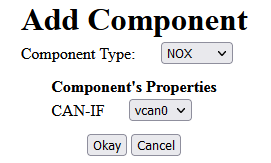
\includegraphics[width=1.5in,angle=0]{../art/Morfeas_web_if/Morfeas_sys_conf_add_comp.png}}
	\caption{Morfeas System add component}
	\label{fig:Morfeas_sys_conf_add_comp}
\end{figure}

\newpage
\subsection{``ISOStandards"}
The ``ISOStandards" show an instance of the current ISOStandard file as table.
The table have five columns with titles: ``NAME", ``DESCRIPTION", ``UNIT", ``MAX", ``MIN".


\begin{lstlisting}[frame=single,caption=Structure of ISOstandard file,label=lst:ISOStandard]
<?xml version="1.0" encoding="UTF-8"?>
<root>
  <points>
    <ISOStandard_name_tag>
      <description>Description of ISOStandard</description>
      <unit>Default Unit</unit>
      <max>Maximum value</max>
      <min>Minumum value</min>
    </ISOStandard_name_tag>
    ....
  </points>
</root>
\end{lstlisting}

\subsection{``Up/DownLoad"}

\begin{figure}[h]
\centering
	\fbox{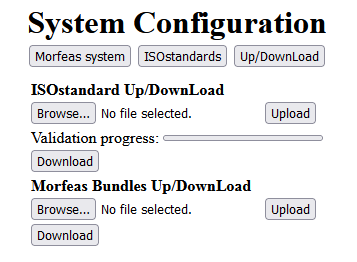
\includegraphics[width=2.5in,angle=0]{../art/Morfeas_web_if/Morfeas_system_conf_up_down.png}}
	\caption{Morfeas System Up/DownLoad}
	\label{fig:sys_conf_up_down}
\end{figure}
